\documentclass[12pt]{article}
\title{\vspace{-2.75cm}On Government Borrowing Behavior\vspace{-0.5cm}}
\author{Nicholas Ray}
\date{\vspace{-0.30cm}December 15 2022\vspace{-1cm}}
\usepackage[utf8]{inputenc}
\usepackage[margin=1in]{geometry}
\usepackage{mathtools,amssymb,amsthm}
\usepackage{setspace}
\usepackage{tikz}
\usepackage{sgame}
\doublespacing
\usepackage[colorlinks,citecolor=cyan,urlcolor=blue,bookmarks=false,hypertexnames=true]{hyperref}
\usepackage[backend=biber, style=authoryear, maxbibnames=99, uniquelist=false]{biblatex}
\renewbibmacro{in:}{}
\renewbibmacro*{volume+number+eid}{%
  \printfield{volume}
  \setunit*{\addnbthinspace}
  \printfield{number}
  \setunit{\addcomma\space}
  \printfield{eid}}
\DeclareFieldFormat[article]{number}{\mkbibparens{#1}}
\AtEveryBibitem{
  \clearfield{issn}
  \clearfield{month}
  \clearfield{urlyear}
  \clearlist{language}
  \clearfield{note}
  \ifentrytype{online}{}{
    \clearfield{url}
  }
}
\DeclareCiteCommand{\citeyear}
    {\usebibmacro{prenote}}
    {\bibhyperref{\printfield{year}}\bibhyperref{\printfield{extrayear}}}
    {\multicitedelim}
    {\usebibmacro{postnote}}
\DeclareCiteCommand{\citeyearpar}[\mkbibparens]
    {\usebibmacro{prenote}}
    {\bibhyperref{\printfield{year}}\bibhyperref{\printfield{extrayear}}}
    {\multicitedelim}
    {\usebibmacro{postnote}}
\addbibresource{ForeignAid.bib}
\begin{document}
\maketitle
\begin{abstract}
    In this proposal, I argue that the observed variation in borrowing behavior by recipient countries in Africa can be explained by the dissonant conditionalities associated with Chinese and Western loans. Autocracies, who find it more costly to accept Western loans due to the West's historical emphasis on liberal political reforms, accept Western loans at an inefficiently low rate and forgo potentially lower conditions stemming from Chinese loan competition. I test the hypothesis that African autocracies have higher proportions of Chinese loans to World Bank loans but do not find support for the statistical importance of regime type. GDP per capita, though, seems to be inversely related with the ratio of Chinese loans to World Bank loans.  
\end{abstract}
\vspace{0.5cm}
\textit{Keywords}: Global Finance, China, World Bank, Africa, Regime Type

\section*{Introduction}
Since engaging in a ``going out'' strategy around the turn of the century, the People's Republic of China (China) has successfully become the ``lender of first resort'' for developing countries \parencite[1]{dreher2022}.\footnote{All R code, data, and \LaTeX \;code underlying my analysis can be found in the corresponding repository on GitHub at https://github.com/nnray.} There has been an abundance of scholarly work attempting to understand the potential effects of China's contemporary prominence in the global finance arena. Much of this literature focuses on how the international financing behavior of more traditional, Western donors have been affected (e.g., \cite{humphrey2019}; \cite{kilama2016a}) or how the effectiveness of their money has changed (e.g., \cite{blair2022}; \cite{gehring2022}).

Little of this work, however, has looked at how the behavior of recipients of international finance has updated since the availability of Chinese money. This lack of attention is despite recent work that implies that recipient countries may extract benefits from their loan choices in a more Chinese global finance environment. While the literature suggests that recipients stand to gain from receiving both Chinese and Western finance and the subsequently more competitive terms, observations of borrowing practices in Africa do not seemingly reflect that recipients are engaging in a strategy to leverage competition between lenders.

Understanding the debt composition of developing countries is an increasingly important issue as public debt continues to rise. This research could also shed light on literature concerned about China's interaction with the liberal international order (LIO) and spark a new research agenda studying recipient behavior.

In the next section I detail what observation is currently not explained and why it should be. My explanation and hypothesis follows. I then introduce my research design and present preliminary results before moving to a discussion of limitations and contributions of the paper.

\section*{What Demands Explanation and Why}
There is evidence that African countries are offered fewer loan conditions from the World Bank (\cite{hernandez2017}) and that Western aid is less sensitive to policy and institutional quality (\cite{annen2021}) when they are recipients of Chinese finance. Although Dreher et al. (\citeyear{dreher2021}) did not find that the effectiveness of aid from the United States (U.S.) is negatively affected by the presence of Chinese aid, their results do suggest that U.S. aid effectiveness increases in the absence of Chinese aid. In sum, this evidence intimates that Western entities are changing their international financial behavior in response to China in a way that benefits recipients.

There is also tentative evidence that China reciprocates these actions. Dreher et al. (\citeyear{dreher2018}) find that Chinese finance increases with Western development assistance, which they interpret as competitive behavior from China (p. 190). Taken together, the literature seems to imply that there is some financial competition between the West and China that recipients may be able to take advantage of to procure more favorable borrowing terms in the future. If recipients value better loan terms (i.e., lower conditionality) and are willing to take on more debt, it seems that it is optimal for recipients to borrow from both the West and China to stimulate competition and induce lower conditions from at least the West. While this logic stemming from the literature does not stipulate a precise proportion of Western to Chinese debt that optimizes recipient benefits, it should at least not be the case that countries borrow almost exclusively from one or the other. Interrogatively, do African countries borrow from the West and China in a way to benefit from their competition? Equivalently, do African countries have debt compositions largely comprised of both Chinese and Western loans?

A cursory view of African debt suggests that this is not universally the case. The proportion of Chinese loans to Western loans varies substantially between counties and, further, some countries almost entirely borrow from either China or the West when taking money from governments. For example, according to information from a charity focused on alleviating debt across the world, the estimated composition of public debt in Cabo Verde and Djibouti nicely reflects this relative reliance on either the West or China (Table 1 and 2, \cite{jubileedebtcampaign2018}). Cabo Verde owes only 1\% of its estimated total debt to China while Djibouti can attribute 68\% of its estimated debt to China, by contrast.

\begin{table}
    \centering
    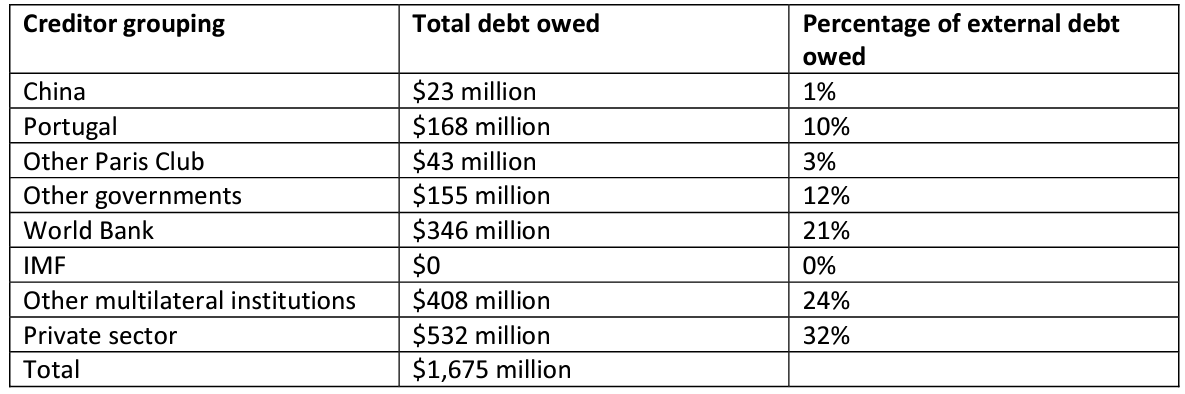
\includegraphics[scale=0.5]{Figures/CaboVerde.png}
    \caption{Estimated Debt for Cabo Verde}
    \vspace{1cm}
    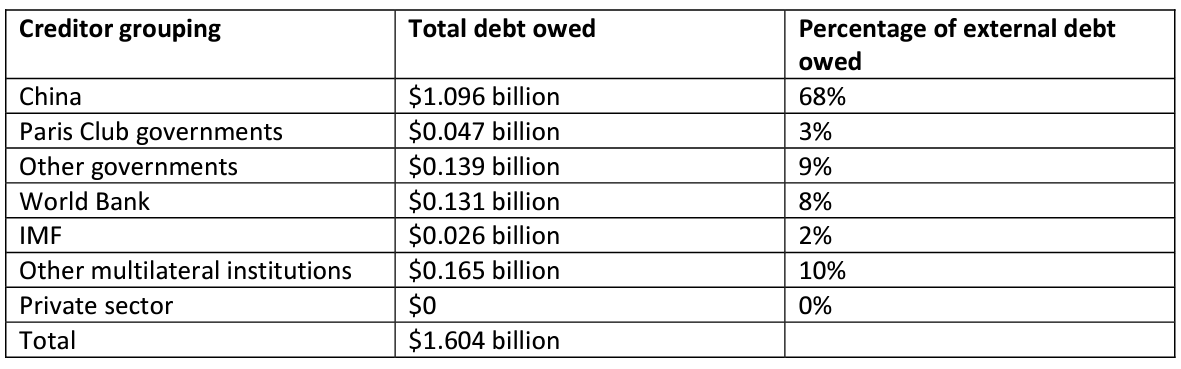
\includegraphics[scale=0.5025]{Figures/Djibouti.png}
    \caption{Estimated Debt for Djibouti}
\end{table}

I gathered observational data from the World Bank (\cite{theworldbankgroup2022a}) and AidData (\cite{custer2021}) to look myself at the sum of loans received from both the World Bank and China for every African country from 2000-2017, as displayed in Table 3. I also provide information from the World Bank (\cite{theworldbankgroup2022}) on the public debt that each country carries. The table reveals a few apparent patterns. For one, World Bank loans seem to be much more common than those from China and, secondly, that the total amount of loans received from the World Bank is relatively constant across countries per a few exceptions (e.g., Namibia). Thirdly, there is extensive variation in the total amount of loans received from China. Some countries take none (e.g., Sao Tome and Principe), while others only consume Chinese finance relative to that from the World Bank (e.g., Equatorial Guinea). In conclusion, when focusing only on the World Bank and China, there is indication that some African countries take finance entirely from the West, others entirely from China, and others still borrow substantially from both (e.g., Botswana).

\begin{table}
    \centering
    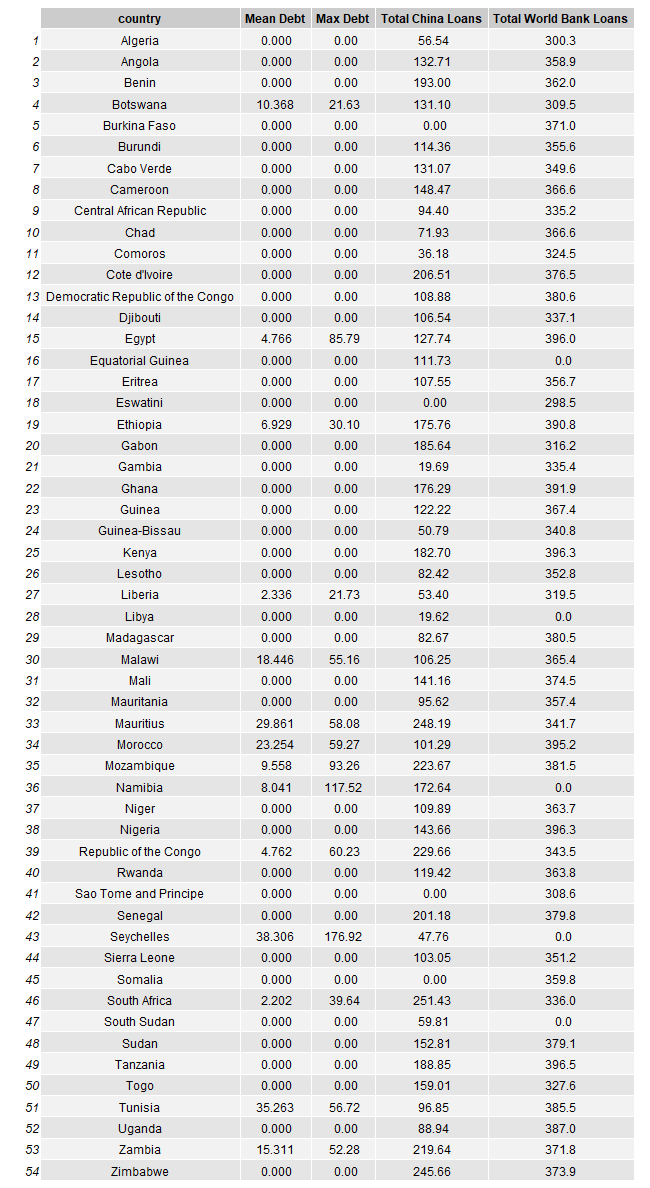
\includegraphics[scale=0.53]{Figures/summary1.png}
    \caption{Summary Table of Debt and Loans in Africa}
\end{table}

Thus, the variance in debt composition and seeming failure of countries to stimulate and benefit from competition by borrowing in a more equal manner between China and Western entities must be explained. In other words, why do some African countries almost exclusively borrow from either the West or China? While there may be little reason to suspect strategy in the reception of foreign aid and grants, it is more puzzling why countries may not optimize their costly loan intake. Recipients presumably want to minimize the costs associated with borrowing money. Related literature, though, seems to not have fully considered recipient decision-making with regard to choosing a borrower, instead largely focusing on macroeconomic and political determinants of government debt in general (e.g., \cite{bittencourt2015} ; \cite{swamy2015}) or the determinants of lender behavior (e.g., \cite{dreher2018}).

\section*{My Explanation}
I argue that the variation observed in African borrowing practices is a result of strategic considerations on behalf of recipients, where countries borrow differently due to dissimilarities in the conditions of Western and Chinese loans and subsequent evaluations of loan value. Specifically, I argue that Western loans typically specify more political conditions and that, therefore, autocratic countries find it more preferable to borrow mostly from China despite the potential financial efficiency gains of incorporating more Western loans.

There is evidence to support the notion that conditionality differs between Chinese loans and those from the West. China seems simultaneously strict on economic conditions (e.g., \cite{dreher2018}; \cite{theeconomist2022}) while being more lax about the political conditions imposed (e.g., \cite{dreher2018}). Western loans, by contrast, seem at least equally strict on the political dimension versus the economic (\cite{hernandez2017}). 

All else equal ($ceteris\;paribus$), rational recipient countries should prefer to accept loans that have less strict conditions. %Why? What are some ways in which loan conditions are consequential?
Further, $ceteris\;paribus$, more autocratic countries should prefer loans that attach fewer political conditions relative to their democratic counterparts. %Why? Be detailed. Usually entails liberal reforms.
It should therefore be more costly for autocratic countries to accept loans from the West compared to democratic countries. 

I argue that, in the short term, this cost outweighs the expected benefit for autocrats of accepting more competitive Western loans and that, subsequently, autocratic countries should have a higher ratio of Chinese loans to those Western compared to democratic countries. This argument generates the following hypothesis:
\begin{align*}
    H_{1}&:\;\text{Autocracies have a higher ratio of Chinese loans to Western loans}\\
\end{align*}

Anecdotally, this story fits with the motivating examples of Cabo Verde and Djibouti, who have Polity scores of 10 and 3 in 2020, respectively (\cite{marshall2018}).
This explanation might also corroborate Dreher et al.'s (\citeyear{dreher2018}) finding that Chinese loans seem to flow to more corrupt countries and those with poorer political institutions.

\section*{Research Design}
To test this hypothesis I collected observational data on all African countries from the years 2000 to 2017. This includes previously discussed data used for Table 3 (government debt, \cite{theworldbankgroup2022}; Chinese loans, \cite{custer2021}; and World Bank loans, \cite{theworldbankgroup2022a}), data on regime type from Polity (\cite{marshall2018}), and gross domestic product (GDP) per capita (\cite{unitednationsstatisticsdivision2019}). A summary of these variables can be found in Tables 4 and 5.

To create a ratio of Chinese loans to Western loans, my dependent variable, I divided logged amounts of Chinese loans by logged amounts of loans from the World Bank. Values less than one for this variable indicate more World Bank loans than Chinese, while higher values than one indicate the opposite. Polity score is my main explanatory variable while GDP per capita is a potential confounder. I regressed this ratio on the Polity score and GDP per capita for each country in the sample, choosing a two-way fixed effects model after finding it superior to a pooled or random effects model. Clustered standard errors by country were also used. The results are presented in Table 6. 

\section*{Preliminary Results}
The results suggest that GDP per capita is inversely related to the ratio of China loans to World Bank loans, implying that richer countries have smaller ratios of Chinese loans to World Bank loans. The main explanatory variable, Polity scores, is not significant at conventional levels, but does have the hypothesized sign (i.e., countries that are more autocratic and with lower Polity scores should be observed to have larger ratios of Chinese loans to World Bank loans). Therefore, there is no support for $H_1$ in the preliminary analysis. 

\begin{table}
    \centering
    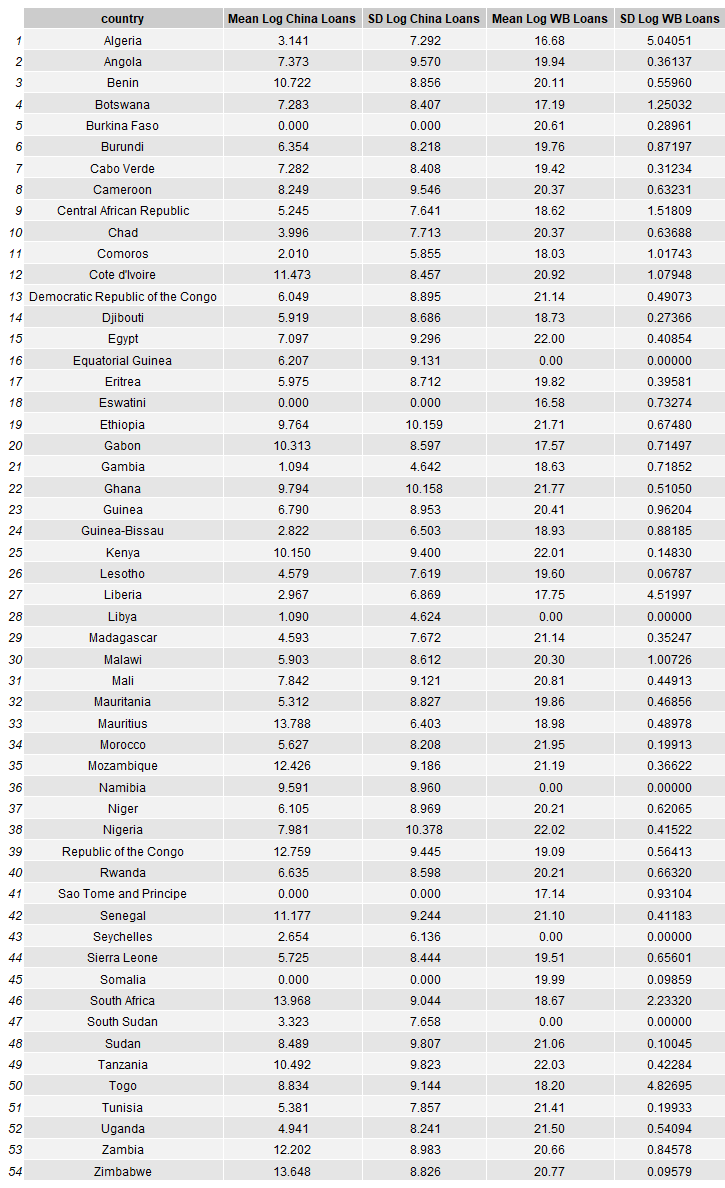
\includegraphics[scale=0.53]{Figures/summary2.png}
    \caption{Summary Table of Variables}
\end{table}

\begin{table}
    \centering
    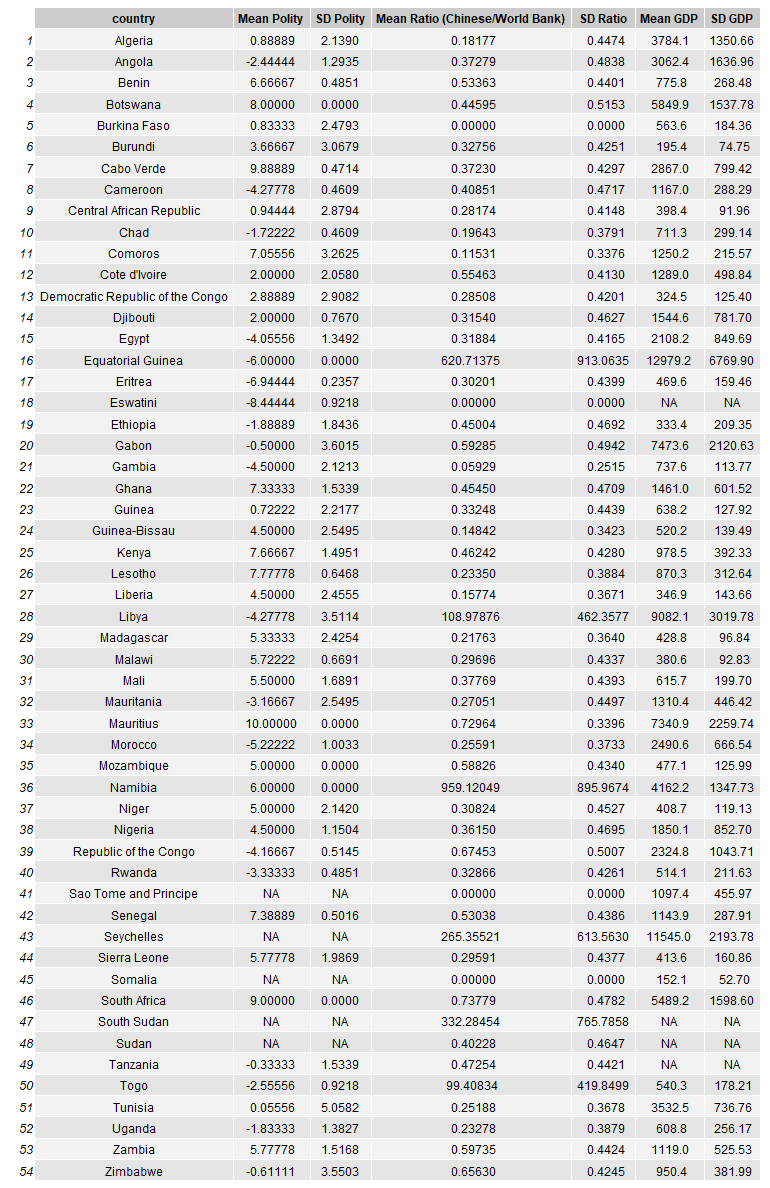
\includegraphics[scale=0.53]{Figures/summary3.png}
    \caption{Summary Table of Variables}
\end{table}

\begin{table}[!htbp] \centering 
  \caption{Accounting for Variation in the Ratio between Chinese and World Bank Loans} 
  \label{} 
\begin{tabular}{@{\extracolsep{5pt}}lc} 
\\[-1.8ex]\hline 
\hline \\[-1.8ex] 
 & \multicolumn{1}{c}{\textit{Dependent variable:}} \\ 
\cline{2-2} 
\\[-1.8ex] & Ratio (China/World Bank) \\ 
\hline \\[-1.8ex] 
 GDP per capita & $-$0.030$^{***}$ \\ 
  & (0.007) \\ 
  & \\ 
 Polity & $-$1.379 \\ 
  & (4.243) \\ 
  & \\ 
\hline \\[-1.8ex] 
Observations & 874 \\ 
R$^{2}$ & 0.024 \\ 
Adjusted R$^{2}$ & $-$0.059 \\ 
F Statistic & 9.792$^{***}$ (df = 2; 805) \\ 
\hline 
\hline \\[-1.8ex] 
\textit{Note:}  & \multicolumn{1}{r}{$^{*}$p$<$0.1; $^{**}$p$<$0.05; $^{***}$p$<$0.01} \\ 
\end{tabular} 
\end{table} 

\pagebreak
\section*{Limitations and Future Improvements}
There exist numerous improvements that must be made to this article. Theoretically, my proposed relationship is intimately related with time, though this is not yet operationalized in my hypothesis or fully included in the theoretical specification. I also need to develop more implications to empirically evaluate and discuss alternative explanations for the alleged unexplained observation of extreme debt composition variation. 

Empirically, I need to specify a better measure for the dependent variable. As it stands, the proposed ratio has two main drawbacks: Firstly, it does not have an upper-bound and thus over-emphasizes countries that receive more Chinese loans than Western loans (i.e., when World Bank loans are close to zero for a particular country, the ratio may go to infinity); Secondly, it only compares loans in single years, not across all the years observed. This means that a country can have a high ratio in a single year (i.e., more Chinese loans accepted than World Bank loans) but in reality have a low ratio over all years observed (i.e., in sum they accepted more World Bank loans than those from China). Further, there is an abundance of missing data for different measures that I need more time to deal with, perhaps via imputation.

In addition, the main explanatory variable (Polity scores) does not have much variance across the years observed. Thus, it is not surprising that it does not account for much of the variation in the dependent variable (loan ratio), which itself has unnecessary variation built-in (since it can have extremely large values with comparatively little meaning). I would like to specify multiple measures of regime type and engage in numerous robustness checks for all variables. 

\section*{Discussion and Conclusion}
While treated trivially in the past, I have argued that the evolving international financial competition in Africa has rendered recipient strategy an important question due to possible, unprecedented benefits they can receive from such competition. Autocracies, who find it more costly than democracies to take loans from the West due to traditionally high political conditions, continue to inefficiently diversify their debt composition between the West and China and do not actualize the potentially lower conditions that recent loan competition has induced. However, my early empirical results do not support the hypothesis that autocracies have larger loan ratios (i.e., China loans/World Bank loans) than democracies.
 
Ideally, this article would be among the first to detail the importance of recipient behavior in the global finance literature. Understanding recipient behavior, instead of only engaging with the study of lenders and powerful countries, may shed light on the political and economic complexity unfolding in Africa and give clues to those concerned about the rising public debt occurring across the continent. Scholars must pay attention to the recipient motivations for accepting loans in addition to lenders' geopolitical motivations in offering them. 

I also contribute to the literature on the liberal international order (LIO), which is engaged in a debate on how China's recent prominence will affect the current LIO (e.g., \cite{weiss2021a}). China seems focused on increasing its global influence via growing its politico-economic ties with developing countries dissatisfied with the LIO (e.g., \cite{broz2020}), and understanding which developing countries have incentives to cooperate with China could be an important piece in calculating China's ability to build its influence and undermine the LIO, should that be what its true aim is. \nocite{leppert2021} \nocite{curini2020}

\pagebreak
\printbibliography
\end{document}